\chapter{Considerações finais}

	\par Conclusão do trabalho. 

        \begin{verbatim}
    	    \begin{ilustracao}[ht]
        		\centering
        		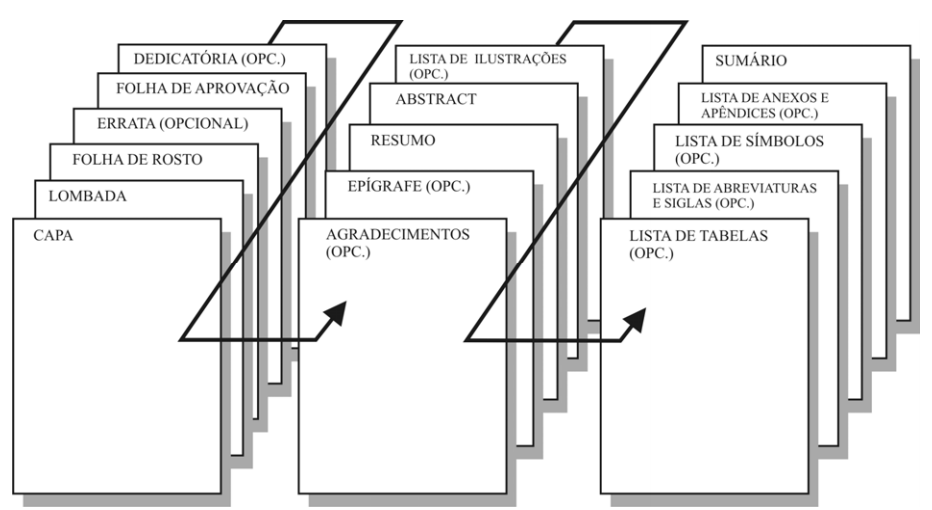
\includegraphics[width=0.6\textwidth]{figuras/pretextuais.png}
        		\caption{\label{exepretex} Sequência dos elementros pré-testuais da MDT-UFSM}
        		\vspace{\baselineskip} %%% linha em branco para atendender a norma
    		\fonte{Adaptado de \citeonline{man:MDTUFSM2012}.}
    	    \end{ilustracao}
        \end{verbatim}
         
         \begin{ilustracao}[ht]
     	    \caption{\label{exepretex} Sequência dos elementros pré-testuais da MDT-UFSM}
	    \centering
	    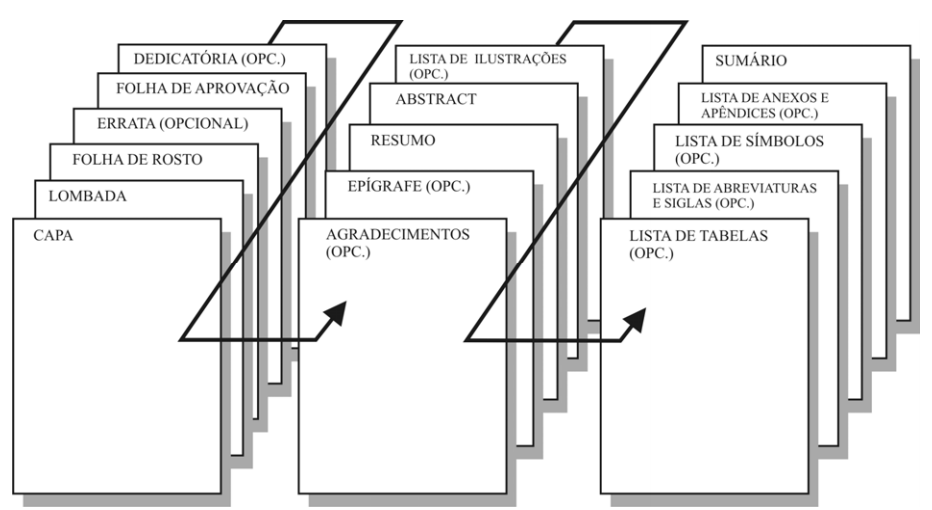
\includegraphics[width=0.6\textwidth]{figuras/pretextuais.png}
	    \vspace{\baselineskip} %%% linha em branco para atendender a norma
            \fonte{Adaptado de \citeonline{man:MDTUFSM2012}.}
         \end{ilustracao}